\section{解析と結果}

\subsection{チェレンコフ角の計算方法}


\begin{figure}
  \centering
  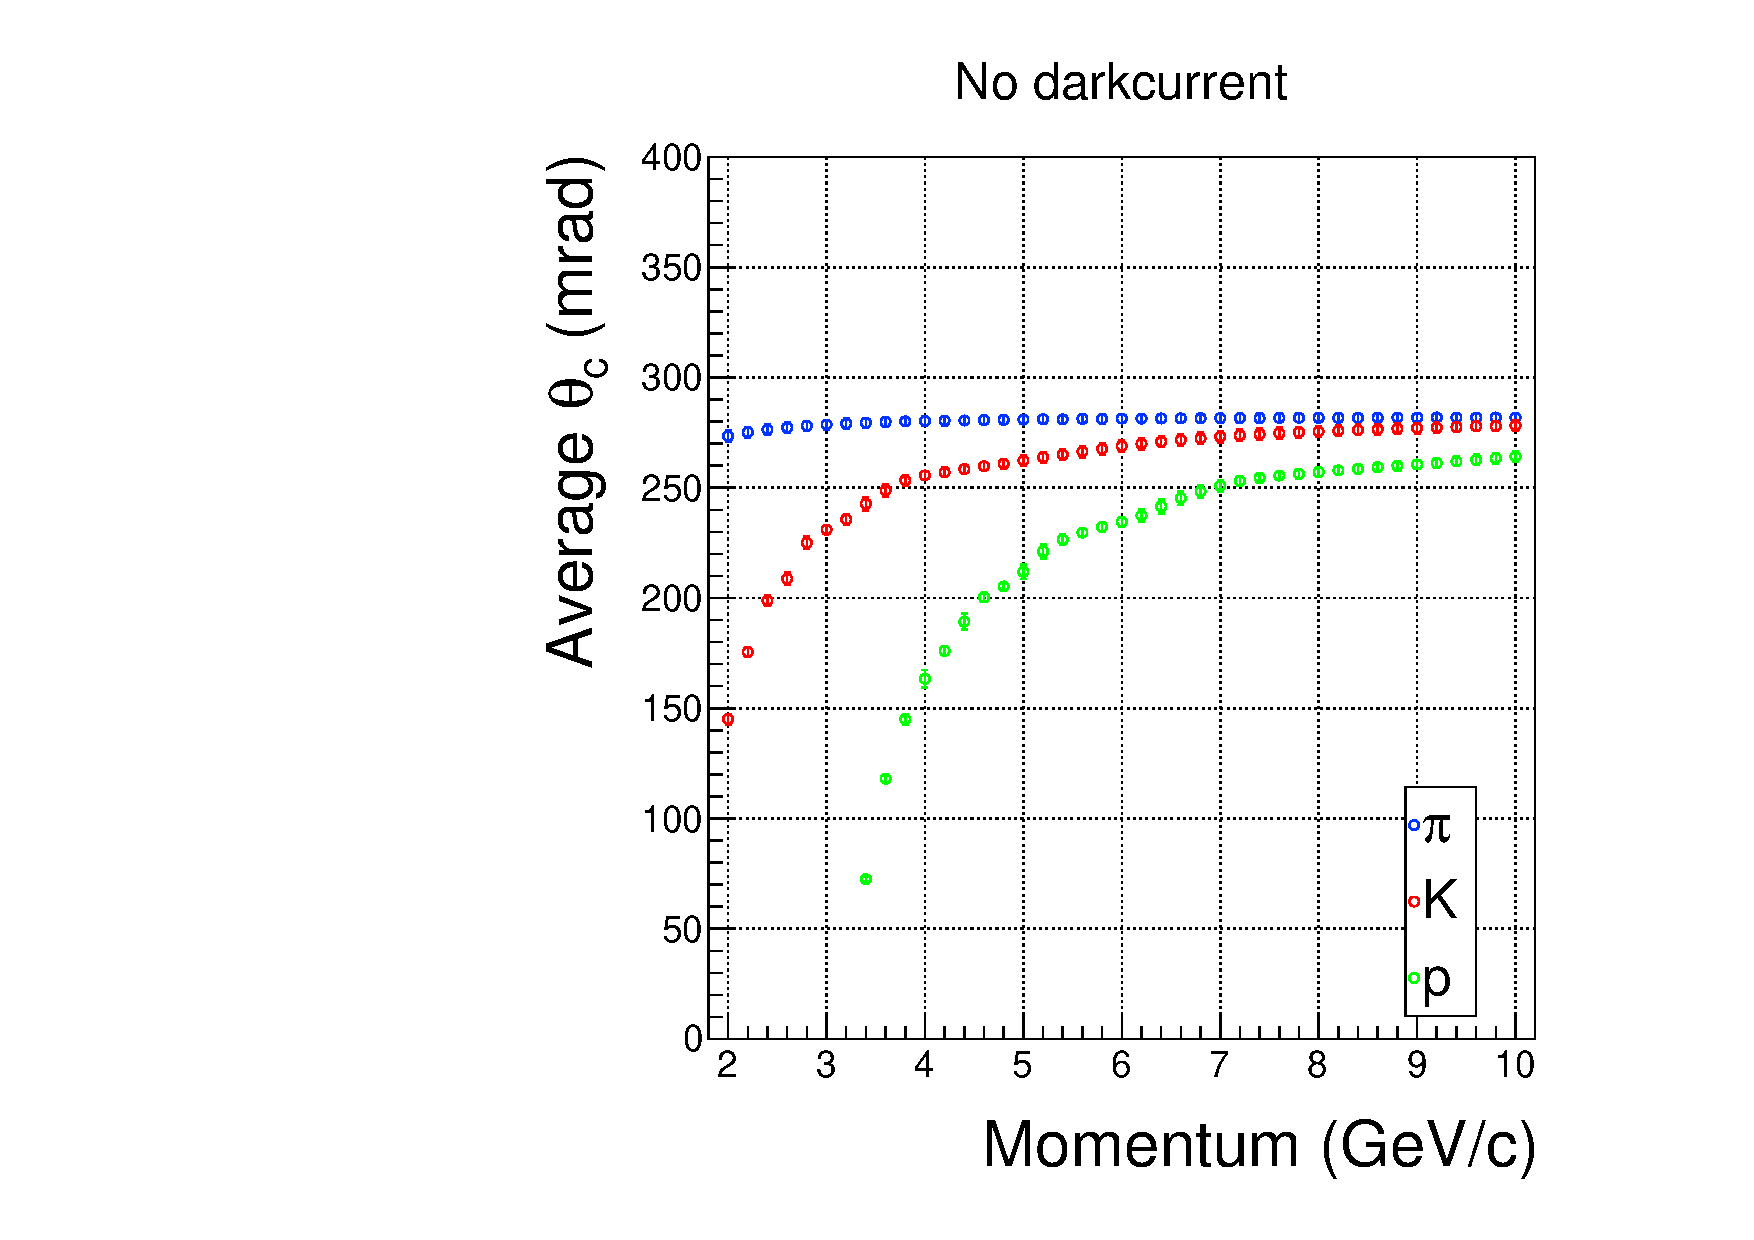
\includegraphics[width=15cm,page=1]{images/chapter4/angleAndMultiGraph.pdf}
  \caption{
    暗電流を考慮しない場合の運動量毎のチェレンコフ角分布。青い点が$\pi$、赤い点がK、緑の点がpを示す。
    エラーバーはチェレンコフ角の分布をガウスフィットした際の$1\sigma$(角度分解能)としている。
  }
  \label{fig:angleMultiGraph1}
\end{figure}

\begin{figure}
  \centering
  \includegraphics[width=15cm,page=2]{images/chapter4/angleAndMultiGraph.pdf}
  \caption{
    暗電流を考慮した場合の運動量毎のチェレンコフ角分布。青い点が$\pi$、赤い点がK、緑の点がpを示す。
    エラーバーはチェレンコフ角の分布をガウスフィットした際の$1\sigma$(角度分解能)としている。
  }
  \label{fig:angleMultiGraph2}
\end{figure}

\begin{figure}
  \centering
  \includegraphics[width=15cm,page=29]{images/chapter4/angleAndMultiGraph.pdf}
  \caption{
    暗電流を考慮しない場合の分離度。青の点が$\pi$/K、赤の点がK/p、緑の点がp/$\pi$の分離度を表す。
    暗電流なしだと、2$-$6\space$\si{GeV/c}$の$\pi$/K、2$-$10\space$\si{GeV/c}$のK/pどちらも$3\sigma$以上分離できている。
  }
  \label{fig:angleMultiGraph3}
\end{figure}
\begin{figure}
  \centering
  \includegraphics[width=15cm,page=30]{images/chapter4/angleAndMultiGraph.pdf}
  \caption{
    暗電流を考慮した場合の分離度。青の点が$\pi$/K、赤の点がK/p、緑の点がp/$\pi$の分離度を表す。
    暗電流ありだと、ほとんどの運動量領域において$2\sigma$以上分離できていない。
  }
  \label{fig:angleMultiGraph4}
\end{figure}